\chapter{薄板型抗震阻尼器数值模拟分析}
在本章中对工程应用中常见的三种薄板型抗震阻尼器进行介绍,随后通过数值建模对其进行数值模拟分析,分别使用三种不同的本质边界条件施加方法罚函数法、Nitsche法和本文所提的基于Hellinger-Reissner原理的变分一致性本质边界条件施加方法得出的弯矩云图进行对比分析,进一步证明所提方法在解决工程应用薄板型抗震阻尼器方面具有一定优势。
\section{TADAS阻尼器}
在建筑和工程结构中,振动是一个常见的问题,其可能会导致结构的疲劳破坏等问题,传统方法中通过采用增加结构的刚度或使用液体阻尼器、摩擦阻尼器减小结构的振动响应,然而在传统方法中或多或少的存在有效性不高,经济适用性低等问题。
为了克服传统方法的限制,三角板(TADAS)减振刚度阻尼器被引入,TADAS阻尼器是一种基于能量耗散原理的被动控制装置,通过在结构中引入附加的阻尼力来吸收和耗散结构的振动能量,能够有效地减小结构地的振动幅值和振动周期,从而显著改善结构的振动响应,
并且TADAS阻尼器的设计相对简单,通常由一块或多块金属材料制成,安装简易、价格低廉,是一种在结构工程中广泛应用于减震和控制结构的被动控制装置。\par
图(\ref{TADAS1})为一个带有TADAS阻尼器的实验装置\cite{mohammadi2017,kim2016},为常在道路、住房和城市中心建造的一层框架大比例模型,
该框架高3米,跨度4米,框架柱采用标准的双IPE180型钢材,梁的工字截面由三块$4000\times200\times12mm$的钢板连续焊接而成。支撑体系统一采用双$100\times100\times20mm$角度,柱基座使用销连接。
如图(\ref{TADAS2})所示,TADAS阻尼器中的三角形板的上端设为简支固定,下端施加$P=100000$的力。三角形钢板的材料系数为杨氏模量$E=2\times 10^{11}$、泊松比$\nu=0.3$。
\begin{figure}[H]
    \centering
    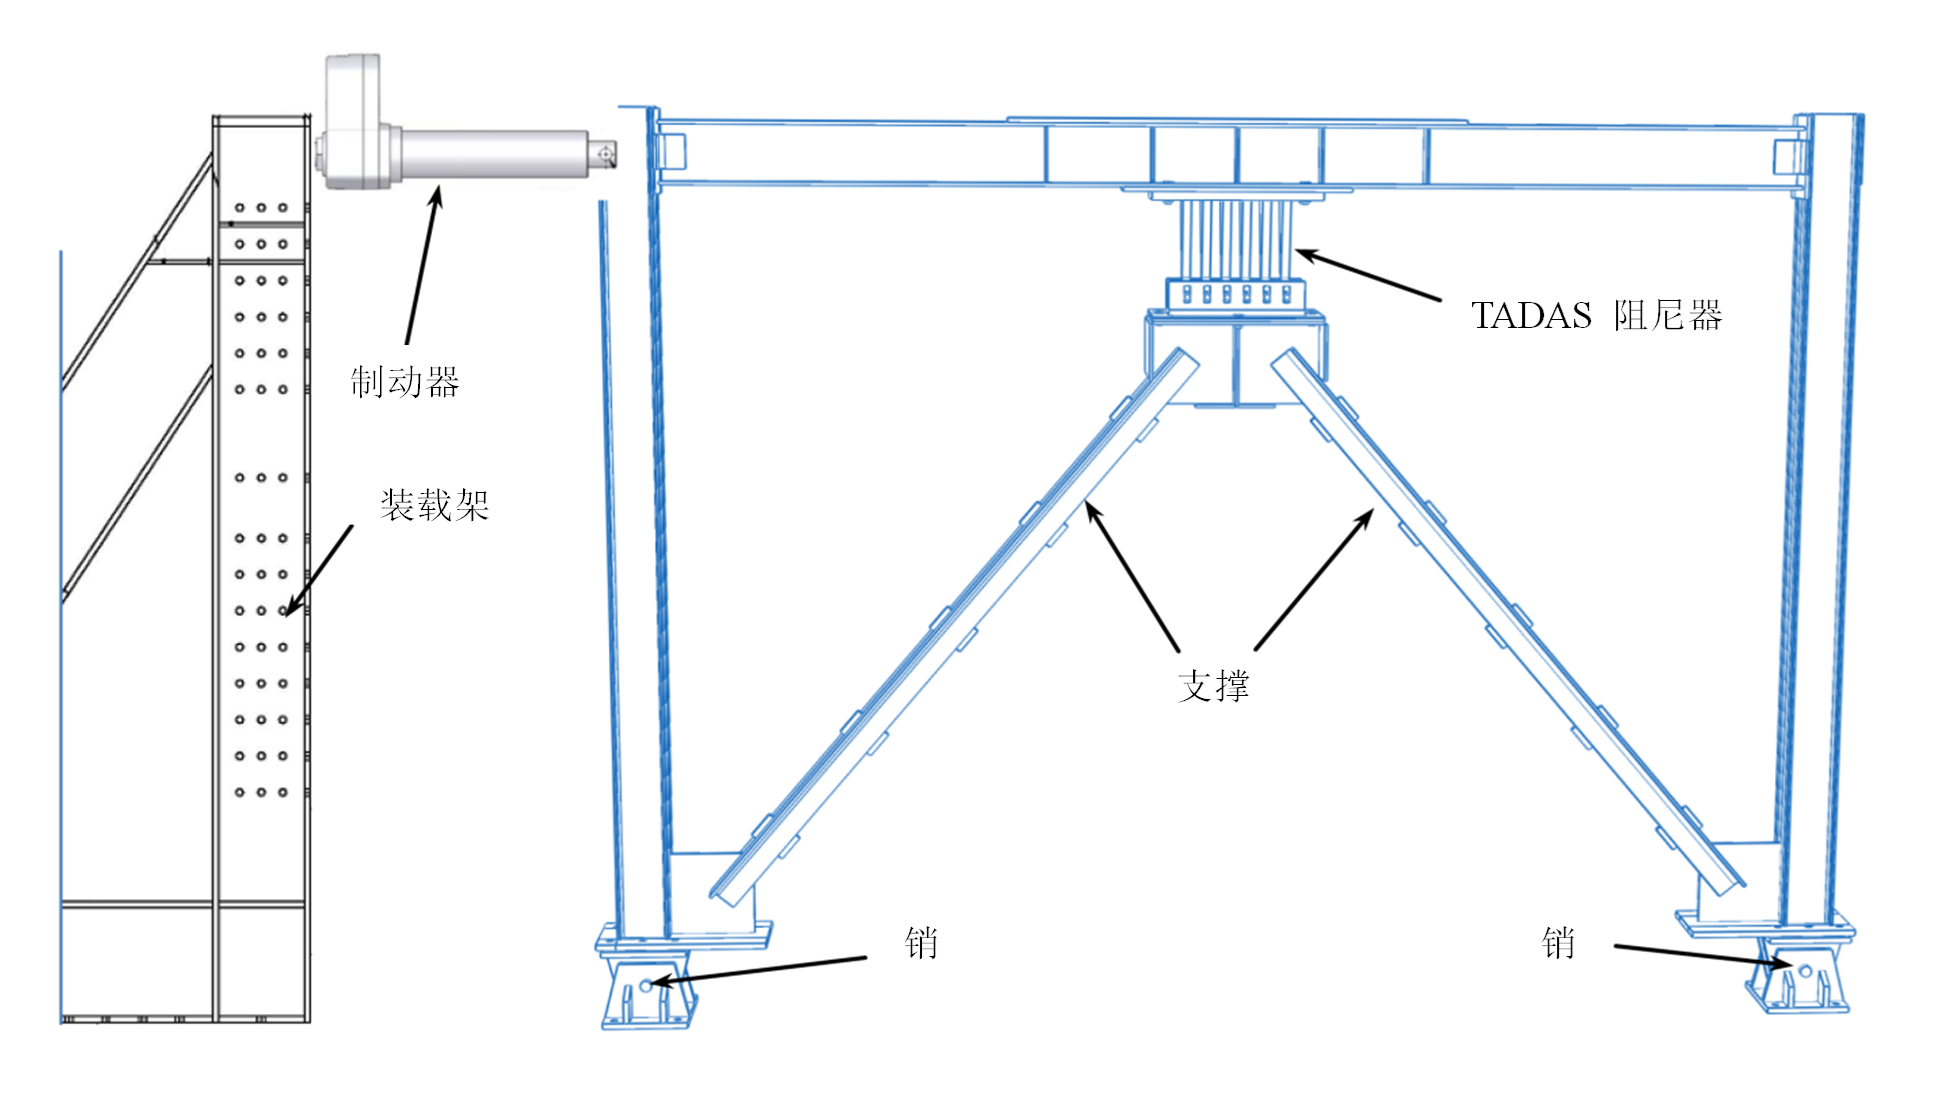
\includegraphics[scale=0.4]{figure/DAMPER/TADAS/1.png}
    \caption{实验装置示意图\cite{mohammadi2017}}\label{TADAS1}
\end{figure}
\begin{figure}[H]
    \centering
    \begin{subcaptiongroup}
            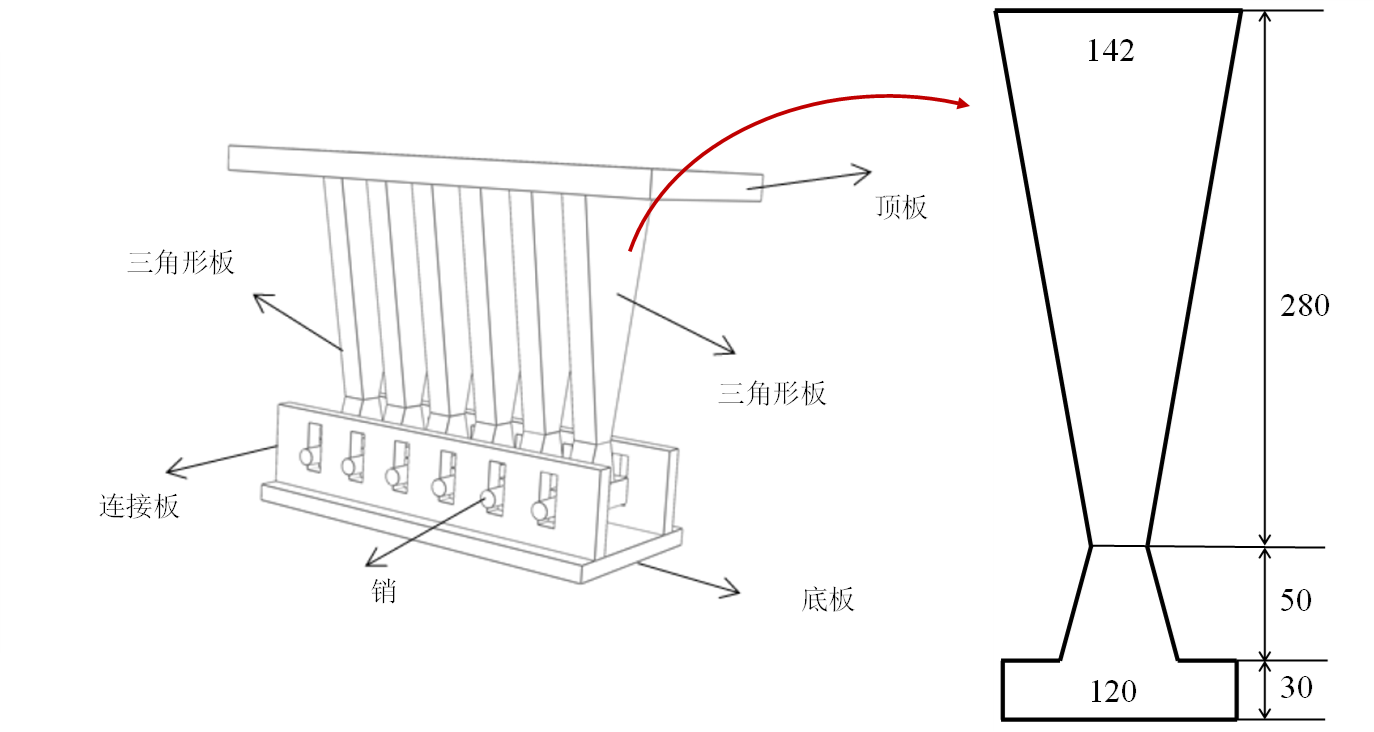
\includegraphics[width=0.69\textwidth]{figure/DAMPER/TADAS/2.png}
            \phantomcaption\label{TADAS2}
            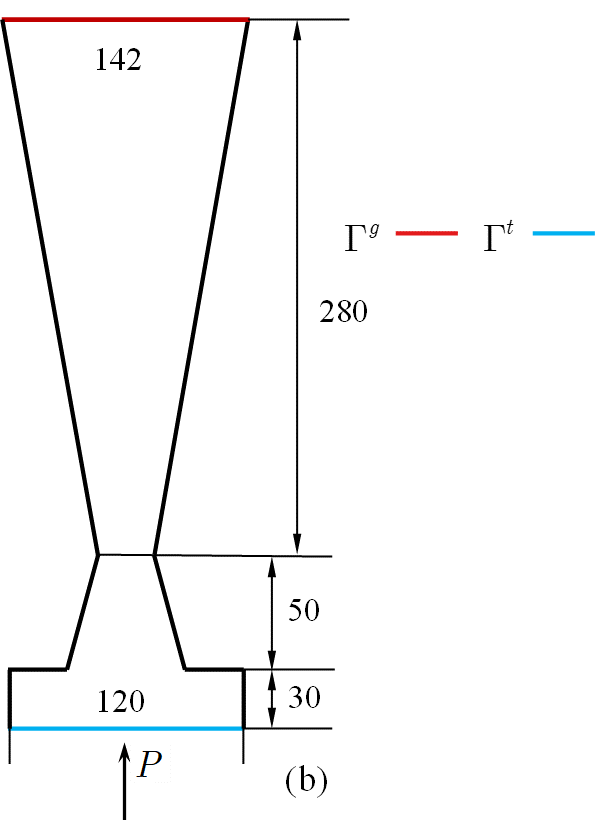
\includegraphics[width=0.29\textwidth]{figure/DAMPER/TADAS/3.png}
            \phantomcaption\label{TADAS3}
            \end{subcaptiongroup}
        \caption{TADAS阻尼器示意图\cite{mohammadi2017}:\subref{TADAS2} 钢板焊接TADAS装置详图;\subref{TADAS3} 三角形钢板横截面图}
    \label{TADAS2}
\end{figure}
图(\ref{TADAS4})为TADAS阻尼器三角形板的弯矩应力云图,从图中可以看出所提方法“RKGSI-HR”法优于“RKGSI-Penalty”、“RKGSI-Nitsche”法。
\newpage
\begin{figure}[H]
    \centering
    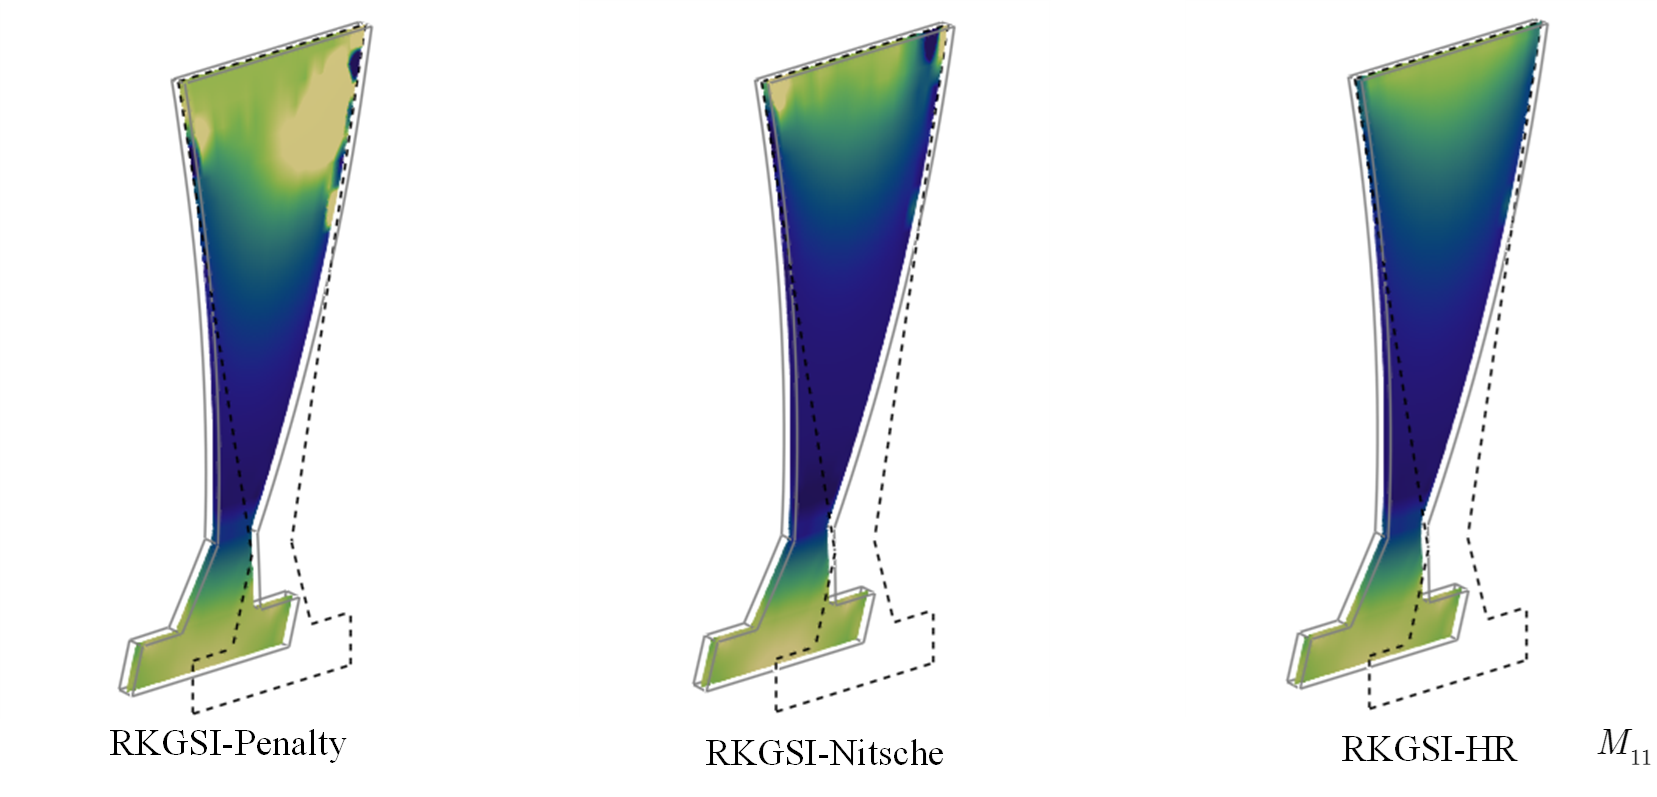
\includegraphics[scale=0.5]{figure/DAMPER/TADAS/M11.png}\\
    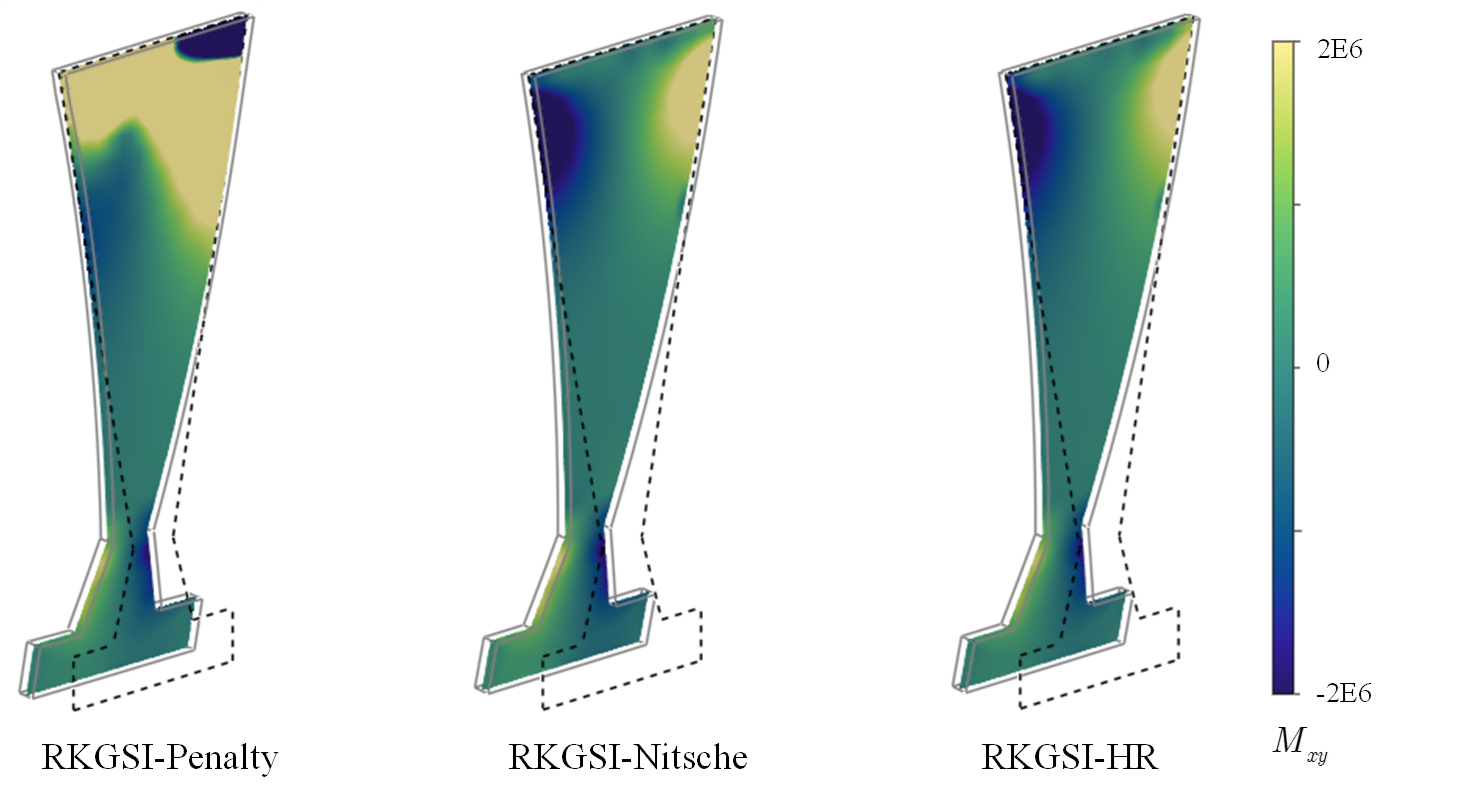
\includegraphics[scale=0.5]{figure/DAMPER/TADAS/M12.png}\\
    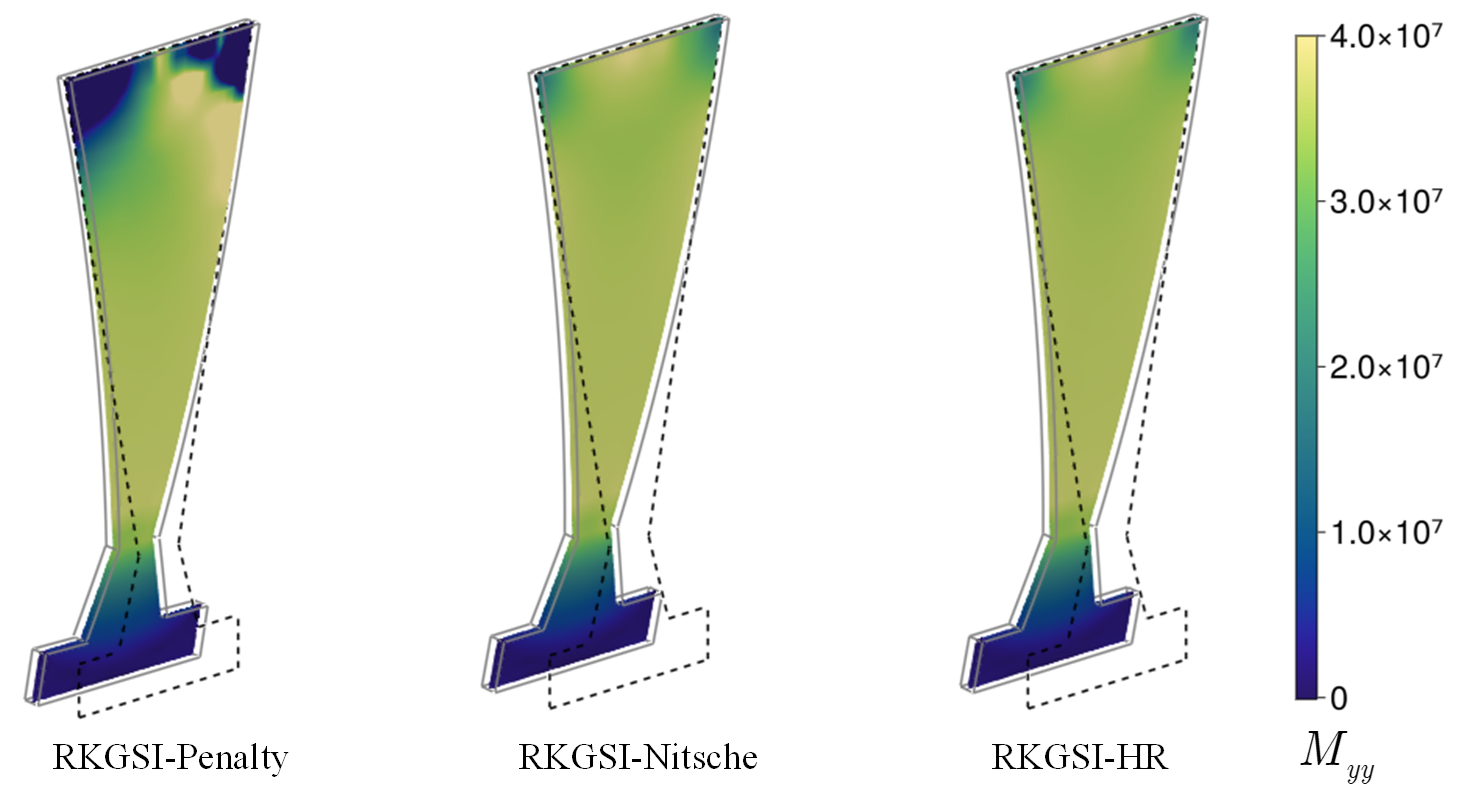
\includegraphics[scale=0.5]{figure/DAMPER/TADAS/M22.png}
    \caption{TADAS阻尼器弯矩云图}\label{TADAS4}
\end{figure}
\section{slit阻尼器}
狭缝(slit)阻尼器通过在建筑结构中引入缝隙,进而吸收和耗散振动能量,从而有效减少结构的振动响应,同时slit阻尼器的结构相对简单,由一系列平行的缝隙组成,可以根据具体的需求进行设计和调整,并且slit阻尼器通常采用钢材或高性能复合材料制造,具有良好的耐久性和抗腐蚀性能,在工程实践应用中越来越广泛。\par
图()为带有slit阻尼器的新型连接体系,梁底部的缝型阻尼器先于主体构件主动塑化,该系统用于震后修复。
如图()所示,为了更好的对slit阻尼器进行受力分析,将slit阻尼器的支板理想化,将圆形的末端替换为直线,对silt阻尼器的上端设为简支固定,下端施加$P=100000$的力。该slit阻尼器的材料系数分别为杨氏模量$E=2\time 10^{11}$、泊松比$\nu=0.3$。
\begin{figure}[H]
    \centering
    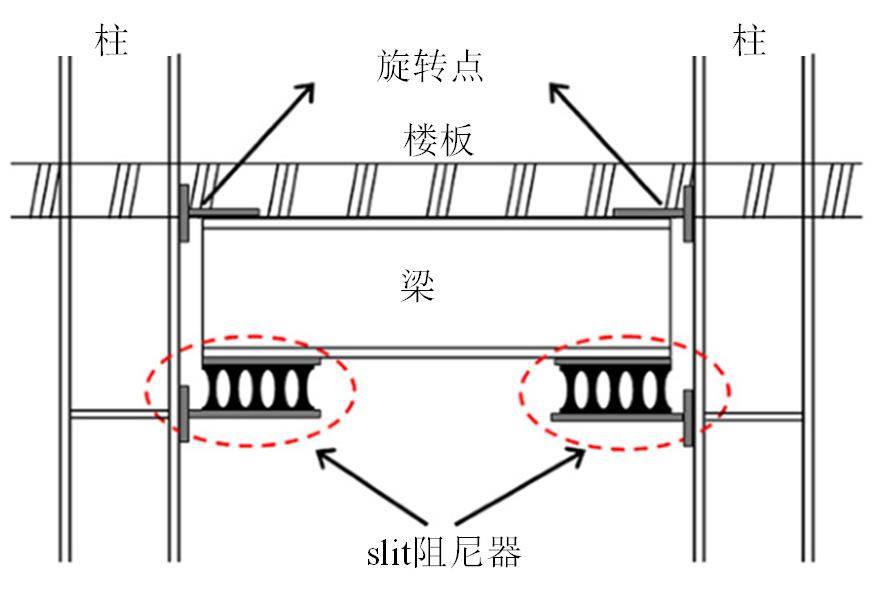
\includegraphics[scale=0.6]{figure/DAMPER/SLIT/1.png}
    \caption{实验装置示意图}
\end{figure}
\begin{figure}[H]
    \centering
    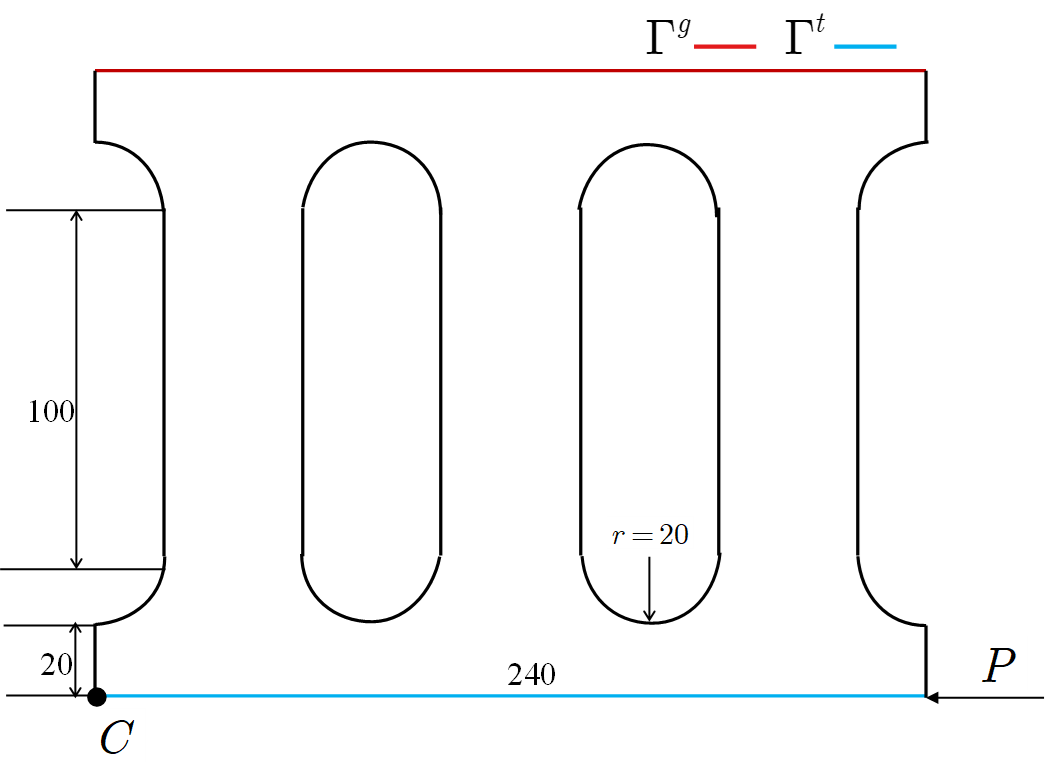
\includegraphics[scale=0.5]{figure/DAMPER/SLIT/2.png}
    \caption{slit阻尼器示意图}
\end{figure}
\section{ADAS阻尼器}
\begin{figure}[H]
    \centering
    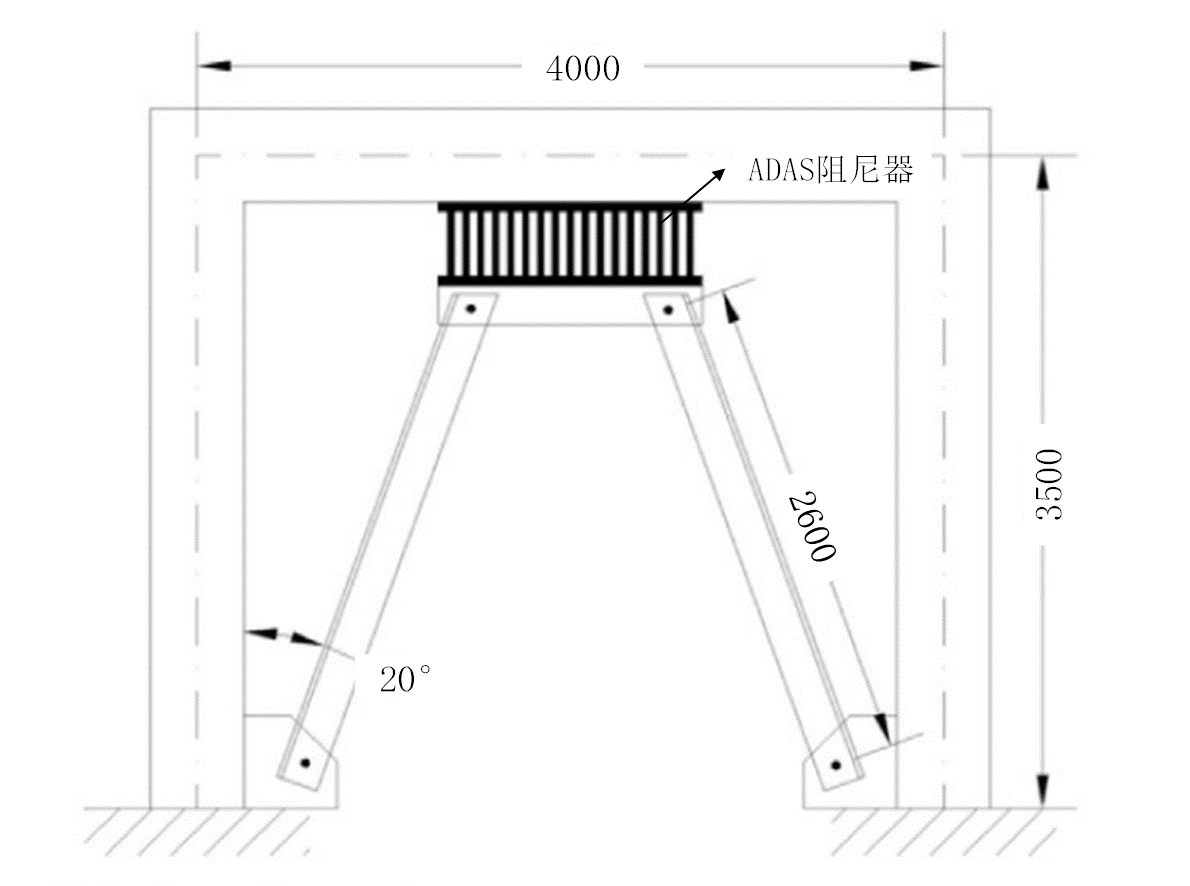
\includegraphics[scale=0.6]{figure/DAMPER/ADAS/1.png}
    \caption{实验装置示意图}
\end{figure}
\begin{figure}[H]
    \centering
    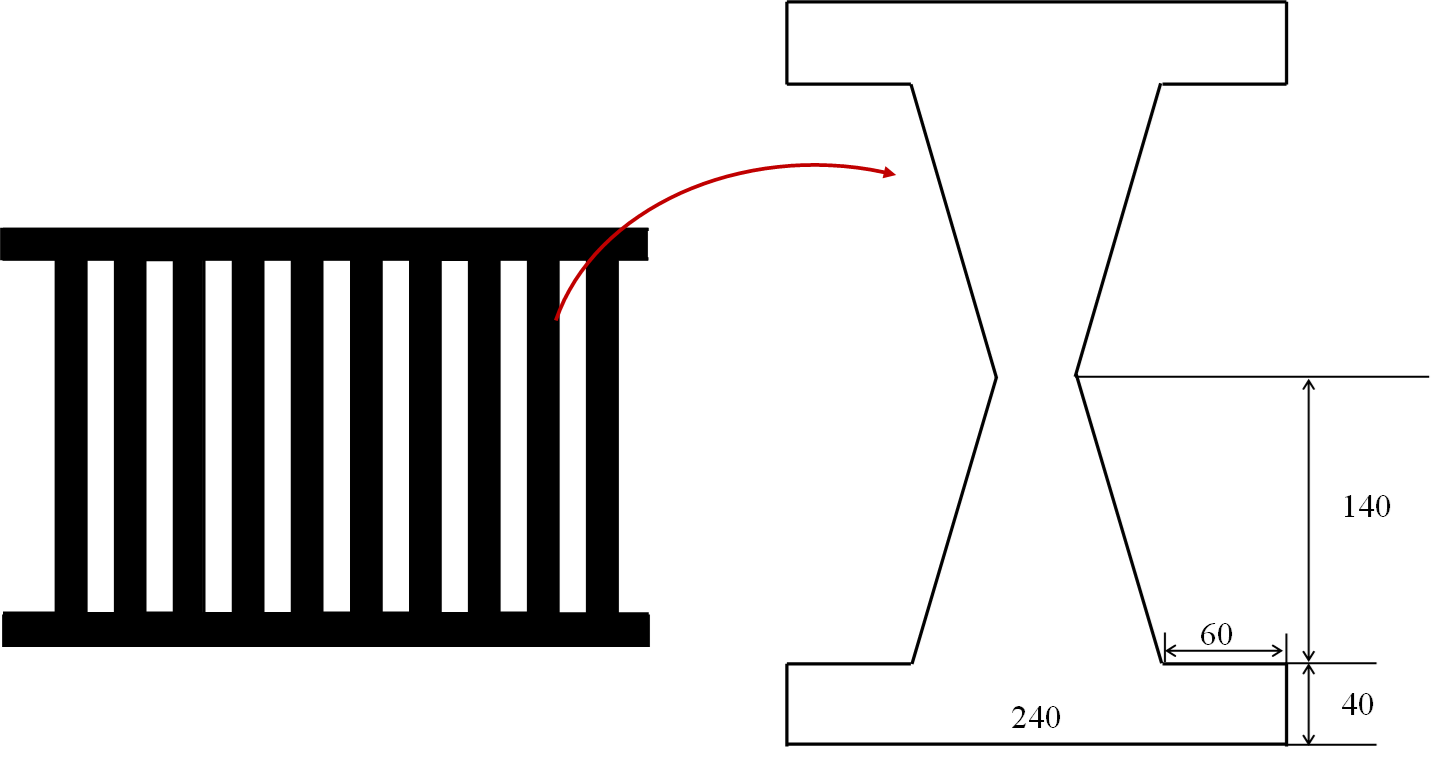
\includegraphics[scale=0.5]{figure/DAMPER/ADAS/2.png}
    \caption{ADAS阻尼器示意图}
\end{figure}
\section{小结}
本章首先对TADAS阻尼器的优点进行详细介绍,随后对一个一层框架大比例模型中带有TADAS阻尼器进行数值分析,通过采用不同的本质边界条件施加方法-罚函数法、Nitsche法和本论文所提方法HR法得到的弯矩云图进行分析,
得出基于Hellinger-Reissner变分原理的变分一致性伽辽金无网格法能够有效处理解决工程实际中的薄板模型,是一种新型的数值分析工具。


